\section{Optimal number of hash functions}

\subsection{Deducing the value of $p'$}
The Bloom Filter is first proposed in~\cite{BF1970} in 1970. Then it is applied in many applications.  Two papers point out that the formula of the false positive of Bloom Filter is wrong. In this paper, we retouch the false positive again:

First, we give the definitions of symbols in Table~\ref{table:symbols}.

\begin{table} [h]
\caption{symbols and their definitions}
\centering
\label{table:symbols}
\begin{tabular}{c c}
\hline symbol & definition \\ 
\hline m & the size of filter \\ 
 	   n & the number of elements \\ 
       k & the number of hash functions \\ 
       S & the set \\ 
       f & the probability of false positive \\
       Q & the number of actions \\ 
       q & how many bits are set in the Q bits \\ 
\hline 
\end{tabular} 
\end{table}

Next we compute the probability of false positive. Same as the original paper, we make two assumptions: 1) $kn<m$; 2) all the hash functions are completely independent and random.

Given a set $S=\{x_1,x_2,... ,x_n\}$, all the elements are mapped into the array with $m$ bits using $k$ hash functions. First we compute $p'$: the probability that one bit of the array is still 0. For one hash, the probability of hashing to the ``one bit'' is $\frac{1}{m}$, then the probability of not hashing to the ``one bit'' is $(1-\frac{1}{m})$. When all the elements are mapped into the array, $kn$ hashing are needed. That one bit of the array is still 0 means that all the $kn$ hashing don't choose it, thus the probability of one bit of the array is still 0 is:

\begin{equation}
\label{p'form}
p'=\left(1-\frac{1}{m}\right)^{kn}
\end{equation}


There is no controversy of the formula of $p'$, the controversy is in the following:

The false positive of Bloom Filter is defined like this: given an element $x$, compute hash values with $k$ hash functions, if all the hash positions are $1s$, it is false positive.
 
The original formula is obtained like this: Given an element $x$, for each hashing, the probability that the hashing position is 1 is $1-p'$ (This is also no problem). Then the probability that all the $k$ hash positions are 1 is $(1-p')^k$. It is known that ``multiple principle'' holds when all the events are independent. As pointed by Prosenjit Bose~\cite{bose2008false}, although the $k$ hash functions are independent, it cannot deduce that the event ``$E(h_1=1),E(h_2=1),E(h_3=1),...,E(h_{i-1}=1)$'' is independent with the event ``$E(h_{i-1}=1)$'', where $E(h_{i-1}=1)$ means the event that the position of $h_{i-1}(x)$ is 1. 

The two papers only said that the judgment ``$E(h_1=1),E(h_2=1),E(h_3=1),...,E(h_{i-1}=1)$'' is independent with the event ``$E(h_{i-1}=1)$'' cannot be deduced, but not tell whether they are independent. We prove they are not independent as follows:

For $k$ hash computations, there are two cases:

1) if all the hashings access the different bits of the Bloom Filters, then the false positive is $(1-p')^k$;

2) if two or more of $k$ hashings access the same bit, the false positive is f'(f'>0).

The overall false positive is $(1-p')^k+f'$, $f'$ bigger than the original formula. 



\subsection{Determine the formula of the optimal $k$}
We need to use the theory of information entropy to deduce the formula of $k$, thus we introduce the basic principle first. 

\textbf{Information Entropy}: In information theory, information entropy is used to measure the uncertainty of a random variable. In this paper, it refers to the \textit{Shannon entropy} \cite{shannon}, which measures the value of the information contained in a message.  Entropy is typically measured in bits, nats, or bans \cite{entropy}. For a variable with $s$ events with the probabilities of $p_1$, $p_2$, ..., , $p_s$. The information entropy is:
\begin{equation}
p'=\sum_{i=1}^{s}p_i  log_2 \dfrac{1}{p_i}
\end{equation}

Here we give some conclusions about information entropy:

%1) 变量的不确定性越大,熵也就越大
1) For a random variable, the larger the uncertainty is, the bigger the information entropy will be. 

2) For any variable or message, there is a maximum value of information entropy.

3) When there are some characteristics or regulations in the message, its information entropy is not the maximum.


Rather than get the exact formula of false positive, given the value of $m$ and $n$, we deduce the exact formula of the optimal $k$ which the two exact formulas cannot get.

According to the theory of information entropy, when there are some characteristics in the array of Bloom Filter, the information entropy is not the maximum, and the array can be still compressed without information loss, which means it is not the optimal value of $k$. In other words, when there is no characteristic (law, information) in the array, its information entropy is the maximum, and the value of $k$ is optimal. Obviously, when the probability of every bit of the array is 0.5, it has no characteristic (law, information), its information entropy reaches the maximum, and the value of $k$ is the optimal - $k^*$:

\begin{equation}
p'=\left(1-\frac{1}{m}\right)^{k^* n}=0.5
\label{equ:p=0.5}
\end{equation}

More strictly, we can compute the information entropy as follows:

\begin{equation}
E=-p'Log_2P'-(1-p')Log_2(1-p')
\end{equation}

We draw the value of E with the increase of $p'$ in Figure \ref{fig:entropy}. Obviously, when $p'=0.5$, the information entropy is maximum of 1. In this way, we can also get equation \ref{equ:p=0.5}.

\begin{figure}
\centering
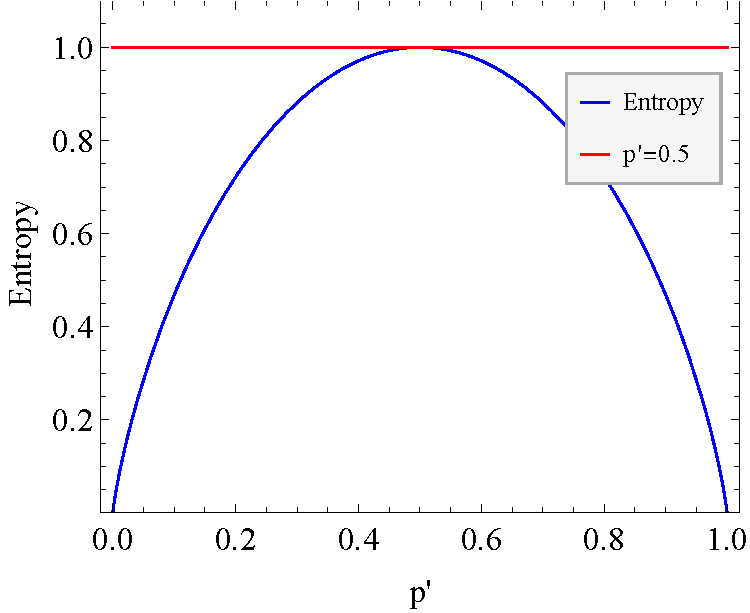
\includegraphics[width=1\linewidth]{entropy}
\caption{Information entropy of Bloom Filters}
\label{fig:entropy}
\end{figure} 

Then we get,

\begin{equation}
\label{kform}
k^*=\dfrac{ln2}{n} \times \dfrac{1}{lnm-ln(m-1)} \approx ln2 \times \dfrac{m}{n}
\end{equation}

As shown in Figure~\ref{eva:err:m}, the difference between 1/(lnm-ln(m-1)) and m fluctuates with a mean of 0.5. When $m$ is large, the difference of 0.5 can be ignored. Equation ~\ref{kform} tells that the exact value of the optimal $k$ is slightly smaller than the original formula. When $m$ is not small, the difference can be ignored.

\begin{figure}
\centering
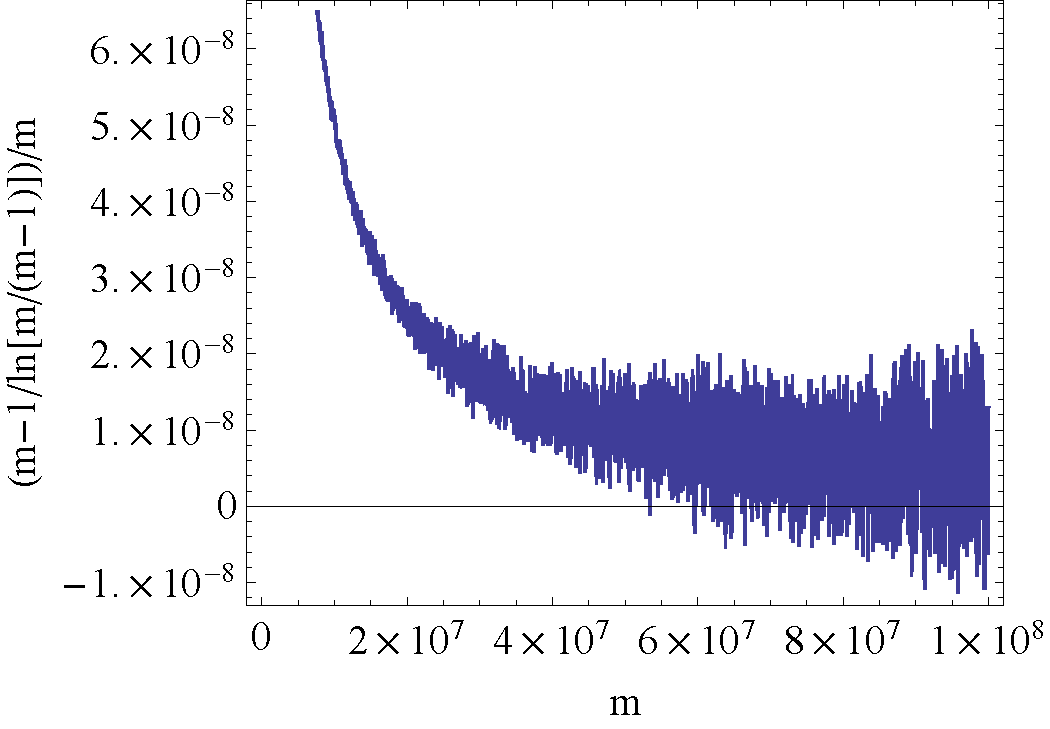
\includegraphics[width=1\linewidth]{error_m}
\caption[FPtest]{error VS. m.}
\label{eva:err:m}
\end{figure} 
%给出k的计算方法
%给出m比较大的时候假阳性计算方法。


\section{Practicality of False Positive Calculation}

\section{The limit form of the probability of Bloom Filter}

To carry out parallel query, the partitioned Bloom Filter is popular. The method of partitioned Bloom Filter is simple: the Bloom Filter is divided into $k$ even partitions, each hash function writes 1s in one partition, respectively. Using this method, there is a characteristic in the partitioned Bloom Filter: each partition of the Bloom Filter has at least one 1.

For partitioned Bloom Filter (pBF), the probability that one bit of the array is still 0 is

\begin{equation}
p'_{partition} = \left( 1-\dfrac{k}{m} \right)  ^n
\end{equation}

Theorem 1: If $m > 1 \;\;,   k >1 \;\; and \;\; n > 1$,

\begin{equation}
\label{theorem1}
\left( 1-\dfrac{k}{m} \right)  ^n < 
\left( 1-\dfrac{1}{m} \right)  ^{kn}
\end{equation}

Proof. 

Let g(k) be $( 1-\frac{1}{m} )  ^k- ( 1-\frac{k}{m} )$, then the derivative of g(k) is:

\begin{equation}
g'(k)=k\left( 1- \dfrac{1}{m}\right) ^{k-1} +\dfrac{1}{m}
\end{equation}

Obviously, when $m > 1 \;\;,   k > 1 $,
g'(k)>0, then we know for any $k > 1$,
g(k)>g(1)=0, thus g(k)>0, according to the assumption kn<m, we can get

\begin{equation}
0<\left( 1-\dfrac{k}{m} \right)   < 
\left( 1-\dfrac{1}{m} \right)  ^k
\end{equation}
When $n \geq 1$, 

\begin{equation}
\left( 1-\dfrac{k}{m} \right) ^n   < 
\left( 1-\dfrac{1}{m} \right)  ^{kn}
\end{equation}

Proof is complete.

According to Theorem 1, we know $p'_{partition} < p'_{true}$, \textit{i.e.}, $1-p'_{partition} > 1-p'_{true}$. This indicates for partitioned Bloom filter, the probability that one bit of the array is 1 is bigger, thus the false positive is also bigger, therefore, we have

%Having characteristic means that the information entropy is not the maximum, thus the probability of false positive $f_{partition}$ is larger than the standard Bloom Filter  $f_{true}$, thus we get

\begin{equation}
f_{partition} > f_{true}
\end{equation}

These two papers tell us that the true value of false positive of Bloom filter $f_{true}$ is larger than the original formula of Bloom $f_{bloom}$, thus we get

\begin{equation}
f_{true} > f_{bloom}
\end{equation}

Then we get

\begin{equation}
\label{bigbig}
f_{partition} > f_{true} > f_{bloom}
\end{equation}

For partitioned Bloom Filter, the probability that one bit of the array is still 0 is:

\begin{equation}
p'_{partition}=\left( 1-\dfrac{k}{m} \right)^n
\end{equation}

Different from standard Bloom Filter, for partitioned Bloom Filter, the event ``$E(h_1=1),E(h_2=1),E(h_3=1),...,E(h_{i-1}=1)$'' is independent with the event ``$E(h_{i-1}=1)$'', where $E(h_{i-1}=1)$ means the event that the position of $h_{i-1}(x)$ is 1, because each hash function is responsible for one partition, and has no effect with each other. Therefore, 

\begin{equation}
f_{partition}=(1-p'_{partition})^k=\left( 1- \left( 1-\dfrac{k}{m} \right)^n \right) ^k
\end{equation}

then the formula~\ref{bigbig} becomes

\begin{equation}
\left( 1- \left( 1-\dfrac{k}{m} \right)^n \right) ^k > f_{true} > \left( 1- \left( 1-\dfrac{1}{m} \right)^{nk} \right) ^k
\end{equation}

Then we use the famous limit formula:

\begin{equation}
\lim\limits_{x \to \infty} \left( 1-\dfrac{1}{x}\right) ^{-x} = e
\end{equation}

and then get

\begin{equation}
\label{flim}
\begin{aligned}
\lim\limits_{m \to \infty} \left(1-\left(1-\frac{1}{m}\right)^{nk}\right)^k  \\ \leq   \lim\limits_{m \to \infty}  f_{true} \leq   \lim\limits_{m \to \infty} {\left(1-\left(1-\frac{k}{m}\right)^n\right)^k }    \\
  \\
 \left(1-e^{-nk/m}\right)^k \leq  \lim\limits_{m \to \infty} f_{true}  \leq  \left(1-e^{-nk/m}\right)^k  \\
\lim\limits_{m \to \infty} f_{true}=\left(1-e^{-nk/m}\right)^k
\end{aligned}
\end{equation}

This gives the limit form of the true false positive of standard Bloom Filter, and it is the same as the original formula. It can be concluded that when $m$ is large, the original formula can be used with negligible error.

Further, we give two vivid examples to show the meaning of \textit{when $m$ is large} as follows:

\subsection{Two Examples}

\textbf{Example 1:}

For example, $m=2, n=1, k=2$, the result using the original formula is 4.5/8.
After hashing, there will be three cases: 10, 01, 11, thus the true false positive is 

\begin{equation}
\dfrac{1}{4}\times \dfrac{1}{4} +\dfrac{1}{4}\times \dfrac{1}{4} +1 \times \dfrac{2}{4}=\dfrac{5}{8}
\end{equation} 

In conclusion, the error is 1/16, when $m$ is 2.


\textbf{Example 2:}
For another example, $m=3,n=1,k=2$, there will be three cases:

Case 1: two hashing map to the same position, the bloom filter array will be one of the three: 100, 010, 001, each with the probability of 1/9. The probability of false positive of Case 1 is: 

\begin{equation}
(\dfrac{1}{3} \times \dfrac{1}{9} ) \times 3 = \dfrac{1}{9}
\end{equation} 

Case 2: two hashings map to different positions, the bloom filter array will be one of the three: 110, 101, 011, each with the probability of 2/9. First we compute the probability of no false positive:

1) Both the first and the second hashing positions are 0, the probability is 1/9.

2) The first hash position is 0, the second hash position is 1, the probability is 
\begin{equation}
\dfrac{1}{3} \times \dfrac{2}{3} = \dfrac{2}{9}
\end{equation} 

3) The first hash position is 1, the second hash position is 0, the probability is also 2/9.

Therefore, the probability of false positive of Case 2 is

\begin{equation}
1-\dfrac{1}{9}-\dfrac{2}{9}-\dfrac{2}{9}=\dfrac{4}{9}
\end{equation}

In sum, the the probability of false positive of Example 2 is:


\begin{equation}
\frac{1}{9}\times 3 \times \frac{1}{9}+ \frac{4}{9}\times 3\times \frac{2}{9}=\dfrac{27}{81}
\end{equation}

Note that the result using the original formula is 25/81, and the error is 2/81.
These two examples imply that the error of the original formulation is very small, and can be ignored when $m$ is not small. 

%套公式得出的结果是 25/81,误差是1/40.5
%
%\subsection{the results of suboptimal value}
%For Standard Bloom Filter (SBF), the probability of false positive is given by:
%
%\begin{equation}
%f=\left(1-\left(1-\dfrac{1}{m}\right)^{nk}\right)^k
%\end{equation}
%
%When m is large, the formula reduces to
%
%\begin{equation}
%\label{math:fpLargem}
%f=\left(1-e^{-\dfrac{nk}{m}}
%\right)^k
%\end{equation}